%%%%%%%%%%%%%%%%%%%%%%%%%%%%%%%%%%%%%%%%%
% Wenneker Assignment
% LaTeX Template
% Version 2.0 (12/1/2019)
%
% This template originates from:
% http://www.LaTeXTemplates.com
%
% Authors:
% Vel (vel@LaTeXTemplates.com)
% Frits Wenneker
%
% License:
% CC BY-NC-SA 3.0 (http://creativecommons.org/licenses/by-nc-sa/3.0/)
% 
%%%%%%%%%%%%%%%%%%%%%%%%%%%%%%%%%%%%%%%%%

%----------------------------------------------------------------------------------------
%	PACKAGES AND OTHER DOCUMENT CONFIGURATIONS
%----------------------------------------------------------------------------------------

\documentclass[11pt]{scrartcl} % Font size

%%%%%%%%%%%%%%%%%%%%%%%%%%%%%%%%%%%%%%%%%
% Wenneker Assignment
% Structure Specification File
% Version 2.0 (12/1/2019)
%
% This template originates from:
% http://www.LaTeXTemplates.com
%
% Authors:
% Vel (vel@LaTeXTemplates.com)
% Frits Wenneker
%
% License:
% CC BY-NC-SA 3.0 (http://creativecommons.org/licenses/by-nc-sa/3.0/)
% 
%%%%%%%%%%%%%%%%%%%%%%%%%%%%%%%%%%%%%%%%%

%----------------------------------------------------------------------------------------
%	PACKAGES AND OTHER DOCUMENT CONFIGURATIONS
%----------------------------------------------------------------------------------------

\usepackage{amsmath, amsfonts, amsthm} % Math packages

\usepackage{listings} % Code listings, with syntax highlighting

\usepackage[spanish]{babel} % English language hyphenation

\usepackage{graphicx} % Required for inserting images
\graphicspath{{images/}{./}} % Specifies where to look for included images (trailing slash required)

\usepackage{booktabs} % Required for better horizontal rules in tables

\numberwithin{equation}{section} % Number equations within sections (i.e. 1.1, 1.2, 2.1, 2.2 instead of 1, 2, 3, 4)
\numberwithin{figure}{section} % Number figures within sections (i.e. 1.1, 1.2, 2.1, 2.2 instead of 1, 2, 3, 4)
\numberwithin{table}{section} % Number tables within sections (i.e. 1.1, 1.2, 2.1, 2.2 instead of 1, 2, 3, 4)

\setlength\parindent{0pt} % Removes all indentation from paragraphs

\usepackage{enumitem} % Required for list customisation
\setlist{noitemsep} % No spacing between list items

%----------------------------------------------------------------------------------------
%	DOCUMENT MARGINS
%----------------------------------------------------------------------------------------

\usepackage{geometry} % Required for adjusting page dimensions and margins

\geometry{
	paper=a4paper, % Paper size, change to letterpaper for US letter size
	top=2.5cm, % Top margin
	bottom=3cm, % Bottom margin
	left=3cm, % Left margin
	right=3cm, % Right margin
	headheight=0.75cm, % Header height
	footskip=1.5cm, % Space from the bottom margin to the baseline of the footer
	headsep=0.75cm, % Space from the top margin to the baseline of the header
	%showframe, % Uncomment to show how the type block is set on the page
}

%----------------------------------------------------------------------------------------
%	FONTS
%----------------------------------------------------------------------------------------

\usepackage[utf8]{inputenc} % Required for inputting international characters
\usepackage[T1]{fontenc} % Use 8-bit encoding

\usepackage{fourier} % Use the Adobe Utopia font for the document

%----------------------------------------------------------------------------------------
%	SECTION TITLES
%----------------------------------------------------------------------------------------

\usepackage{sectsty} % Allows customising section commands

\sectionfont{\vspace{6pt}\normalfont\scshape} % \section{} styling
\subsectionfont{\normalfont\bfseries} % \subsection{} styling
\subsubsectionfont{\normalfont\itshape} % \subsubsection{} styling
\paragraphfont{\normalfont\scshape} % \paragraph{} styling
\setlength{\parskip}{6pt}

%----------------------------------------------------------------------------------------
%	HEADERS AND FOOTERS
%----------------------------------------------------------------------------------------

\usepackage{scrlayer-scrpage} % Required for customising headers and footers

\ohead*{} % Right header
\ihead*{} % Left header
\chead*{} % Centre header

\ofoot*{} % Right footer
\ifoot*{} % Left footer
\cfoot*{\pagemark} % Centre footer
 % Include the file specifying the document structure and custom commands

%----------------------------------------------------------------------------------------
%	TITLE SECTION
%----------------------------------------------------------------------------------------

\title{	
	\begin{center}
		
\includegraphics[scale=0.4]{itba-logo}
	\end{center}
	\vspace{25pt} % Whitespace
	\normalfont\normalsize
	\textsc{Instituto Tecnológico de Buenos Aires}\\ % Your university, school and/or department name(s)
	\vspace{25pt} % Whitespace
	\rule{\linewidth}{0.5pt}\\ % Thin top horizontal rule
	\vspace{20pt} % Whitespace
	{\huge Informe Trabajo Práctico Especial}\\ % The assignment title
	\vspace{25pt} % Whitespace
	{\huge Criptografía y Seguridad [72.44] - 2021 1C}\\ % The assignment title
	\vspace{12pt} % Whitespace
	\rule{\linewidth}{2pt}\\ % Thick bottom horizontal rule
	\vspace{12pt} % Whitespace
}

% \author{\LARGE Grupo 16: Luciano Boccardi - Tamara Puig -  Ximena Zuberbuhler} % Your name

\author{
  Boccardi, Luciano (59518)\\
  \texttt{lboccardi@itba.edu.ar}
  \and
  Puig, Tamara (59820)\\
  \texttt{tpuig@itba.edu.ar}
  \and
  Zuberbuhler, Ximena (57287)\\
  \texttt{xzuberbuhler@itba.edu.ar}
}

\date{\normalsize\today} % Today's date (\today) or a custom date

\begin{document}

\maketitle % Print the title

%----------------------------------------------------------------------------------------
%	FIGURE EXAMPLE
%----------------------------------------------------------------------------------------

\newpage

\section{Recuperación del Secreto}

\begin{figure}[h] % [h] forces the figure to be output where it is defined in the code (it suppresses floating)
	\centering
	\fbox{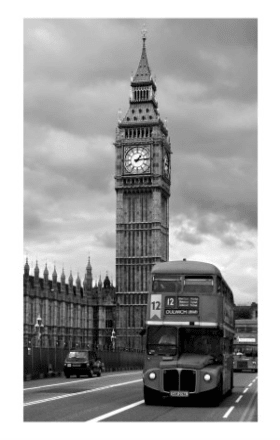
\includegraphics[width=0.5\columnwidth]{big-ben.png}}
	\caption{Imágen recuperada a partir de los archivos dados.}
	\label{secret_image}
\end{figure}

%------------------------------------------------

\subsection{Conclusiones de la ejecución del programa}

El archivo asignado al grupo consistía de 4 imágenes BMP. Se recuperó el secreto con un esquema de 4 imágenes portadoras y el resultado fue la imagen mostrada en la \figurename{\ref{secret_image}}. Habiendo seguido el algoritmo de manera correcta, se puede concluir que la recuperación fue efectiva.

%----------------------------------------------------------------------------------------
%	TEXT EXAMPLE
%----------------------------------------------------------------------------------------

\section{Decisiones de implementación}

\subsection{Manejo de imágenes BMP}

\subsubsection{Distribución}

Cuando se corre el programa en modo distribución, se implementa un límite de $N = 100$ shadows, que es la cantidad de espacio reservado para cada estructura correspondiente a las shadows que se mantiene en memoria. Todas las imágenes primero se leen, luego se cargan a memoria, se procesan y se sobreescriben las imágenes correspondientes.

En cuanto al almacenamiento, en la consigna se había recomendado procesar las imágenes de la siguiente manera (consideremos un esquema simple, de $4x4$):

$$
\begin{bmatrix}
12 & 13 & 14 & 15 \\
8 & 9 & 10 & 11 \\
4 & 5 & 6 & 7 \\
0 & 1 & 2 & 3
\end{bmatrix}
$$

No obstante, se decidió por facilidad de implementación guardar los bytes en el orden que se leen y accederlos de manera inversa:

$$
\begin{bmatrix}
0 & 1 & 2 & 3 \\
4 & 5 & 6 & 7 \\
8 & 9 & 10 & 11 \\
12 & 13 & 14 & 15
\end{bmatrix}
$$

Esto altera la forma de obtener los bloques, pero es transparente para la implementación porque se implementaron métodos que abstraen esa lógica, devolviendo el bloque correspondiente al subíndice que se requiera.

Cuando más de un valor de X se repite, se va sumando 1 operando en $Mod$ $256$ para evitar que hayan valores repetidos entre las shadows. Cuando se excede de 255 se vuelve al número 0, en lugar de restar desde el mayor número. Esto es netamente una decisión de implementación contra un tradeoff de ''ruido'' en las portadoras.

\subsubsection{Recuperación}

Para la recuperación, la forma de lectura es similar a la implementada en la distribución. Se toman exactamente $k$ imágenes del directorio, la cual no es aleatoria, sino son las primeras $k$ que resultan del recorrido.

En lo que corresponde al procesamiento, ante cualquier error en el bit de paridad se termina la ejecución del programa con el código y el mensaje de error correspondientes.

La consideración respecto a la recuperación es que la imagen secreta toma el header correspondiente a la primer sombra que fue leída, y guarda el secreto recuperado con el nombre que fue pasado como argumento para el programa. En el caso de que ya exista un archivo previamente creado con el mismo nombre y en el mismo path, se sobreescribe.

\subsection{Interpolación}

Para la interpolación es necesario realizar el cálculo de los inversos multiplicativos. Esto se puede hacer programáticamente o de manera estática (considerando que el polinomio generador se mantiene constante. En este caso decidimos mantener el cálculo estático. Se asignó un valor para el inverso multiplicativo de 0, esto NO IMPLICA que dicho número posea un inverso multiplicativo. Es solo por comodidad en el acceso a los valores indexados en el array.

\subsection{Información extraordinaria}

Se añadió un parámetro de $--verbose$, su objetivo es brindar un poco más de información sobre lo realizado por el procesamiento. Es totalmente opcional y su uso fue netamente por motivos de análisis y verificación durante la etapa de resolución del problema.



%----------------------------------------------------------------------------------------
%	TEXT EXAMPLE
%----------------------------------------------------------------------------------------

\section{Cuestiones a Analizar}

\subsection{Discutir los siguientes aspectos relativos al documento}

\subsubsection{Organización formal del documento}

El paper analizado tiene una estructura muy bien organizada. Primero se realiza una mención del estado del arte, y trabajos previos del mismo tema. Luego, se comienza a describir la idea y la teoría que la respalda. Se explican las etapas de encripción y desencripción con diagramas de flujo, lo cual ayuda a comprender el procedimiento. Por último, se detalla la carga útil y se realizan comparaciones con los métodos detallado al comienzo del informe.

\subsubsection{La descripción del algoritmo de distribución y la del algoritmo de recuperación}

En cuanto a la descripción de los algoritmos, si bien es sumamente clara, se encontraron algunos problemas en las fórmulas. Muchos de los signos '-' no aparecen, e incluso en la fórmula 7 está mal detallada ya que refiere a $s_{0}$ y no a $s_{r-1}$ como debería. No obstante, al ser fórmulas correspondientes a un método de interpolación ampliamente conocido, no hubieron mayores inconvenientes. También, la fórmula correspondiente al $Payload$ no tiene a $k$ como variable sino que utiliza el número $4$, pero por el contexto se entiende. El resto es detallado y completo, con un grado de detalle adecuado para poder ser comprendido por personas con una formación correspondiente.

\subsubsection{La notación utilizada}

La notación es correcta, no obstante, los índices a los que se refieren suelen entrar en conflicto con los utilizados en las fórmulas matemáticas. Por ejemplo, se utiliza $j$ para denominar el número de bloque, y en la fórmula de interpolación se itera sobre el índice $q$. Quizás hubiera sido mejor optar por definir otros índices para evitar esos conflictos.

Por último, existe un debate cuestionable entre comenzar a indexar con el número 0 o con el número 1. No nos parece relevante discutir sobre cuál es más adecuado, ya que todo depende del lenguaje en el cual se trabaje. A fines de un paper, es correcto porque se mantiene consistente a lo largo del mismo.

%------------------------------------------------

\subsection{El título del documento hace referencia a que optimiza la carga útil, ¿a qué se refiere?, ¿qué relación existe entre k y el tamaño de la portadora?}

Cuando en el paper se refiere a la carga útil está hablando de cuánta información se guarda en cada sombra. Si asumimos que el bloque (4 píxeles = 4 bytes) es la menor unidad de información, entonces podemos establecer una comparación.

Suponiendo que todas las shadows son del mismo tamaño que coincide con el tamaño del secreto. Sea $k$ el número de sombras y $L$ el tamaño del secreto, la imagen se divide en $\frac{L}{k}$ conjuntos de $k$ elementos. Por cada conjunto, se guarda 1 elemento en un bloque de $2x2$.

Es fácil notar que si $k = 4$, se utilizan $\frac{L}{k} * 4$ píxeles, que es exactamente el mismo tamaño que la imagen original.

En el caso $k > 4$, se puede definir un factor de carga $f = \frac{4}{k}$ que define qué porcentaje de cada imagen se ocupa guardando el secreto. Para $k = 5, f = 0.8$, y para $k = 6, f = 0.67$.

No se menciona la optimización de la carga útil en ningún momento. Pero podemos suponer que tiene que ver con el tamaño de bloque escogido. En bloques de $2x2$ se utilizan los 3 bits menos significativos de 3 píxeles para guardar el valor de F. En bloques más grandes se alteran menos bits a cambio de una menor modificación en los datos de la shadow, con el inconveniente de que aumenta el tamaño mínimo requerido.  

Puede verse que mientras mayor es $k$, se necesitan más portadoras pero el tamaño requerido de cada una para guardar el secreto es menor. Si consideramos que $L$ es, en bytes, la cantidad de datos "secretos", como mínimo para recuperarlos se necesita $4*L$. 

%------------------------------------------------

\subsection{¿Qué ventajas y qué desventajas ofrece trabajar en GF($2^{8}$) respecto de trabajar con congruencias módulo?}

La principal ventaja que ofrece trabajar con campos de Galois GF($2^8$) es que no tiene problema para generar valores en el rango $[0,255]$, lo cual es fundamental para la recuperación de los datos. Es por esto que el algoritmo se puede aplicar para recuperar cualquier tipo de archivo binario, no solo imágenes, sin pérdida de información. Si trabajáramos con congruencias $Mod$ $251$ o $Mod$ $257$ que son los dos primos más cercanos al rango, es explícita la pérdida de datos.

Las desventaja más importante tiene que ver con la dificultad de operar en los campos de Galois, lo cual aumenta la complejidad de las operaciones y hace mucho más difícil el debugging del código. Además, para operar en el campo se necesita conocer el polinomio generador correspondiente. Por ende, dos personas que operen con el mismo algoritmo pero empleen un polinomio distinto, van a obtener resultados inconclusos entre sí.

%------------------------------------------------

\subsection{¿Se puede trabajar con otro polinomio generador? ¿Podría guardarse como “clave”?}

Es posible trabajar con otro polinomio generador. En el paper utilizado para basar este trabajo, para los resultados experimentales, se utilizó como polinomio primitivo el polinomio 
$g(x) = x^8 + x^4 + x^3 + x + 1$ que equivale al número 283, el cual es distinto al utlizado en este trabajo. Lo único importante es considerar que debe ser de orden 8 y mayor a 255.

La idea es utilizar el mismo polinomio generador, que se encuentre dentro de $GF(2^8)$, para la encripción y desencripción de la imagen. Cuando hay más de un polinomio en el algoritmo es necesario saber de antemano cuál es.

Para poder encriptar y desencriptar, es necesario saber de antemano el polinomio generador y el $k$ (cantidad mínima de sombras). Entonces, se podría tomar como ''clave'' algún tipo de combinación entre estos datos. Es decir, el polinomio puede ser parte de una ''clave'' pero también se debería incluir el $k$.

%------------------------------------------------

\subsection{Según el documento se pueden guardar secretos de todo tipo (imágenes, pdf, ejecutables). ¿Por qué? (Relacionarlo con la pregunta 3)}

En el algoritmo se toma una cierta cantidad de bytes como input, se obtiene la función correspondiente para realizar la descomposición en pares $(X, F(X))$. En este caso por un tema correspondiente al tipo de imágenes y el tamaño, se decidió arbitrariamente que el ocultamiento se realice únicamente sobre la sección de los datos de la imagen secreta correspondiente a la matriz de píxeles.

Si en lugar de ocultar solo esa parte, se decide ocultar todo el archivo (Desde el byte $0$ hasta el byte $n$), se podrían ocultar todo tipo de archivos, con la condición de que el esquema y el tamaño de las shadows sea el adecuado. Esto se debe a que, a fin de cuentas, los archivos terminan siendo una sucesión de bytes.

Al extender el algoritmo, tomar una imagen, un archivo PDF o un binario de un programa compilado en C terminaría siendo lo mismo a efectos del algoritmo.

En relación a la pregunta 3, el campo de Galois permite generar valores en el intervalo $[0, 255]$ sin problemas. Esto previene una pérdida de datos que podría ocurrir al trabajar con $Mod$ $251$, por ejemplo, donde ya mencionamos que hay una pérdida efectiva debido a la naturaleza de la operación. En las imágenes utilizar la operación de módulo no representa un gran impacto porque la pérdida de valores no altera la naturaleza del secreto (el color resulta similar), pero esta operación en otro tipo de archivo puede alterarlo o corromperlo.

%------------------------------------------------

\subsection{¿Cómo podría adaptarse la implementación realizada para poder guardar un archivo de imagen completo? (Es decir, guardando encabezado y pixeles)}

Para que la implementación realizada pueda guardar el archivo de la imagen completo, lo único que bastaría cambiar sería:

\begin{itemize}
  \item Pasar por el proceso de encripción y desencripción el archivo completo, no solo los píxeles de la imagen.
  \item Cuando se desencripta, no adjuntarle el encabezado de una imagen camuflaje como se hace actualmente.
\end{itemize}

De igual manera, hay que considerar que el tamaño de las shadows debe ser adecuado como para soportar la carga de dichos datos.

%------------------------------------------------

\subsection{Analizar cómo resultaría el algoritmo si se usaran imágenes en color (24 bits por píxel)}

En el caso que se desee utilizar imágenes a color como imágenes camuflaje, se debe tener en cuenta que, como los píxeles de estas imágenes son de 24 bits en vez de 8, los bloques que se tomarán de las imágenes camuflaje serán de 12 bytes en vez de 4.

Cuando se toma el $X$ para calcular el $F(X)$, se tomará solo el primer byte del píxel. Luego, se esconderá $F(X)$ en los últimos 3 bits del tercer byte de los píxeles $W$, $Y$, $Z$. Solo se alteran 3 bits de 24 en los píxeles $W$, $Y$, $Z$.

Por otro lado, cuando se utilizan imágenes en escala de grises, se terminan alterando 3 bits de 8 en los píxeles $W$, $Y$, $Z$. Como el porcentaje de bits alterados por píxel es menor, las imágenes camuflaje con el secreto ya escondido tienen mejor definición que las imágenes a escala de grises.

%------------------------------------------------
\subsection{¿Se podrían tomar los bloques de otra manera, en lugar de como matrices $2x2$? Explicar}

Si, se podrían tomar bloques con otras dimensiones siempre teniendo en cuenta que la cantidad de bloques totales no puede ser menor a la cantidad de bloques en los que se divide nuestra imagen secreta puesto que de otra quedaría una parte del secreto sin distribuir. 

Por ejemplo podrían tomarse en las shadows matrices de $3x3$, $2x4$ o incluso $1x4$. En el último caso sería análogo a $2x2$ pero con una distribución espacial distinta.

Lo que se va a ver afectado al modificar la forma de seleccionar los bloques es el ruido que existirá una vez ejecutado el algoritmo en las imágenes portadoras. Si se toman bloques de tamaño menor a $2x2$, hay más ruido. Si, por el contrario, se toman bloques más grandes, se alteran más píxeles pero menos bits de cada uno, lo que genera menos alteraciones visuales.

%------------------------------------------------
\subsection{Discutir los siguientes aspectos relativos al algoritmo implementado}
\subsubsection{Facilidad de implementación}

La dificultad de la implementación radicaba en el real entendimiento del algoritmo. Una vez comprendido como funcionaba el mismo su desarrollo era relativamente simple. No existieron funciones complejas ni operaciones que causaran demasiado trabajo a la hora de implementarlo.

Los dos mayores problemas enfrentados durante la implementación fueron: la aritmética en el campo de Galois, que es naturalmente compleja y difícil de debuggear en caso de errores, por lo que hay que proceder con un cuidado importante al momento de realizar las funciones; y la representación de las imágenes en matrices, ya que el orden en que se lee difiere del orden en el cual se trabaja.

\subsubsection{Posibilidad de extender el algoritmo o modificarlo}

El algoritmo se podría extender, por ejemplo, para trabajar con otros tipos de archivos. Sería relativamente simple extender la distribución a otros formatos de archivo, dado que se trabaja con binarios.

Otra extensión del algoritmo posible es aceptar la elección de otro polinomio para el campo de Galois, este debería ser un parámetro de la función, por ejemplo. O, en otro caso, poder ocultarse dentro de los datos a recuperar.

Una modificación posible es alterarlo para trabajar con otro tipo de bloques. Esto sería oportuno en caso de que se precise una cantidad de ruido mucho menor al distribuir el secreto en las imágenes portadoras.

Finalmente, una idea que se nos ocurrió es llevar el algoritmo a una implementación de esteganografía de audio. Es decir, en lugar de ocultar los datos en imágenes del tipo BMP, hacerlo en algún formato de audio adecuado. La idea sería la misma, aprovechar los bits menos significativos para ocultar los mensajes.

%------------------------------------------------
\subsection{¿En qué situaciones aplicarían este tipo de algoritmos?}

Este tipo de algoritmos es especialmente bueno cuando la distribución del secreto se tiene que hacer con una determinada cantidad de partes, y se requiere que al menos un subconjunto de ellas se ''reúna'' para poder recuperar el contenido.

Un ejemplo de esto sería, por ejemplo, una clave de alta seguridad en una empresa o agencia gubernamental. Supongamos que ante una emergencia se debe recuperar dicha clave que fue repartida entre N personas de alta jerarquía, y se establece que se requieren como mínimo K para que se autorice el procedimiento. Esto evita, de manera primaria, problemas de exceso de autoridad.

Otra opción interesante podría ser el traslado de la información por un canal inseguro. Imaginemos que se quiere enviar un archivo binario con información de índole sensible. Utilizar uno de estos esquemas permite, por ejemplo, reducir el potencial riesgo de exponer esta información, siempre y cuando el atacante desconozca que se está empleando el algoritmo. En caso de que el atacante pueda conocerlo, se debe procurar jamás enviar K partes por el mismo medio. Una opción sería enviar K-1 por el medio inseguro, y una de las restantes de manera física (Memoria USB, por ejemplo).

%------------------------------------------------

\end{document}
